\documentclass[./main.tex]{subfiles}

\begin{document}
\section{Models}
The following section covers the architectures of the various models that will be used in Section \ref{sec:experiments} when we will be performing our experiments. 

\subsection{Baseline}
\begin{figure}[htbp]
    \centering
    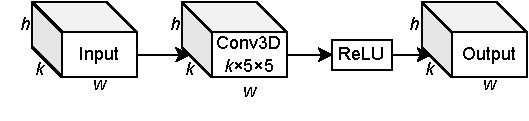
\includegraphics[width=0.8\textwidth]{./entities/baseline.pdf}
    \caption{Illustration of the implemented baseline model.}
    \label{fig:baseline}
\end{figure}

\noindent The first model we will be using in Section \ref{sec:experiments} is a very simple baseline model based on a 3-dimensional convolution. Figure \ref{fig:baseline} illustrates the architecture of the model.
\\
\\
The model takes a sequence of $T \in \mathbb{R}$ estimated poses $\hat{\mathcal{P}} = \{\hat{\bm{P}}^t\}_{t = 1} ^T$ as input, where each estimated pose $\hat{\bm{P}}^t \in \mathbb{R}^{K \times h \times w}$ is represented using heatmaps, such that $K \in \mathbb{R}$ is the amount of keypoints in each estimated pose, $h \in \mathbb{R}$ is the height of each heatmap and $w \mathbb{R}$ is the width of each heatmap.
\\
\\
Once the data has been passed to the model, the processing of the data is very simple. As illustrated in Figure \ref{fig:baseline}, the model starts by applying a 3-dimensional convolutional layer to the input data. The convolutional layer consists of $K$ filters, each with a kernel-size of $T \times 5 \times 5$. To ensure the input and output of the convolutional layer has the same shape, we pad the input with zeros.
\\
\\
Once the convolutional layer has processed the data, the ReLU activation-function is applied element-wise to the data, resulting in the final prediction of the model.

\subsection{Bidirectional Convolutional LSTM}
\begin{figure}[htbp]
    \centering
    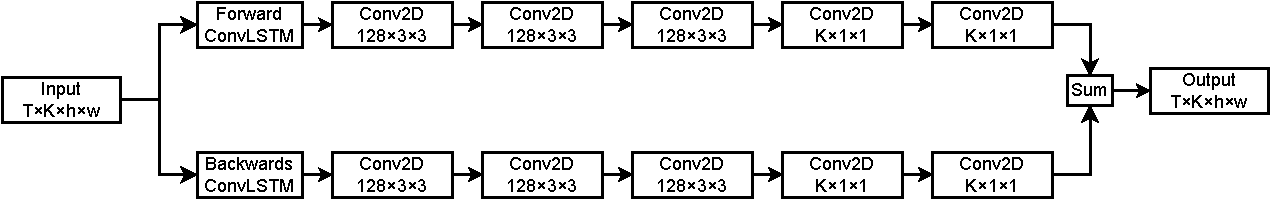
\includegraphics[width=\textwidth]{./entities/bi_conv_lstm.pdf}
    \caption{Illustration of the implemented bidirectional convolutional LSTM}
    \label{fig:bi_conv_lstm}
\end{figure}

\noindent Our second model is a bidirectional convolutional LSTM, inspired by the Unipose-LSTM byArtacho and Savakis \cite{https://doi.org/10.48550/arxiv.2001.08095}. Figure \ref{fig:bi_conv_lstm} illustrates the architecture of the model. The model takes a sequence of $T \in \mathbb{R}$ estimated poses $\hat{\mathcal{P}} = \{\hat{\bm{P}}^t\}_{t = 1} ^T$ as input, where each estimated pose $\hat{\bm{P}}^t \in \mathbb{R}^{K \times h \times w}$ is represented as a set of heatmaps, where $K \in \mathbb{R}$ is the amount of keypoints, $h \in \mathbb{R}$ is the height of each heatmap and $w \in \mathbb{R}$ is the width of each heatmap. 
\\
\\
The model starts by branching into two seperate branches, that processes the estimated poses in opposite sequence order. Each branch processes the estimated poses one frame at a time. This is done by first applying a convolutional LSTM to the input frame at time step $t \in \mathbb{R}$, using the preceding output of the convolutional LSTM as the hidden state. Each convolutional LSTM is followed by five 2-dimensional convolutional layers, each applying $128$ filters, except for the last convolutional layer of each branch, which aplies $K$ filters. The two first convolutional layers use a kernel size of $3 \times 3$, whereas the following two convolutional layers use a kernel size of $1 \times 1$. The outputs of the two branches are then summed together element-wise.
\\
\\
All convolutional layers use a stride of one and zero-padding on the input, such that the output of each convolutional layer has the same dimensions as the input to the convolutional layer.

\subsection{DeciWatch}
\begin{figure}[htbp]
    \centering
    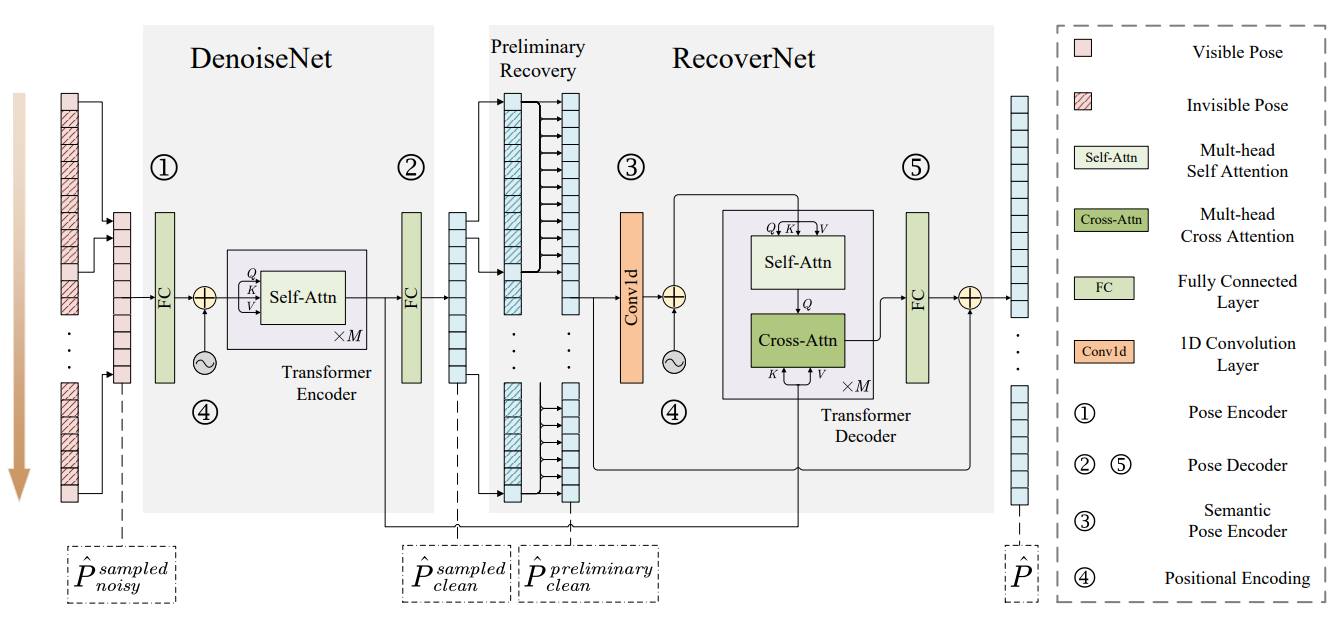
\includegraphics[width=\textwidth]{./entities/deciwatch.PNG}
    \caption{Illustration of the DeciWatch \cite{https://doi.org/10.48550/arxiv.2203.08713}}
    \label{fig:deciwatch}
\end{figure}
\noindent The last model we implement is a transformer-based model named \textit{DeciWatch}, introduced by Zeng \textit{Et al.}, which is illustrated in Figure \ref{fig:deciwatch}. The model works by only processing some of the input-frames. It consists of two parts: the \textit{DenoiseNet} and the \textit{RecoverNet}. The aim of DenoiseNet is to denoise the estimated poses given as input to the model, whereas the aim of RecoverNet is to recover the poses of the missing frames. The following description of the model is based on an interpotation of the official paper behind DeciWatch \cite{https://doi.org/10.48550/arxiv.2203.08713}.
\\
\\
More specifically, the model takes a sequences of $T \in \mathbb{R}$ estimated poses $\hat{\mathcal{P}} = \{\hat{\bm{P}}^t\}_{t = 1} ^T$ as input, where $\hat{\bm{P}}^t$ is represented by 2-dimensional keypoint position. Due to redundancy in consecutaive frames and continuity of human poses, the model starts by sampling every $n$th frame to select sparse poses $\hat{\bm{P}}^{sampled} _{noisy} \in \mathbb{R}^{\frac{T}{n} \times (2K)}$, where $K \in \mathcal{R}$ is the number of keypoints. These sampled poses are then passed to DenoiseNet.
\\
\\
The goal of DenoiseNet is to denoise the sparse poses, that were estimated by a single-frame pose estimator. The denoise process can be formulated as
\begin{equation}
    \hat{\bm{F}}_{clean} ^{sampled} = \textbf{TransformerEncoder} \left( \hat{\bm{P}}_{noisy} ^{sampled} \bm{W}_{DE} + \bm{E}_{pos} \right).
\end{equation}
That is, $\hat{\bm{P}}_{noisy} ^{sampled}$ is first encoded through a linear projection matrix $\bm{W}_{DE} \in \mathbb{R}^{2K \times C}$ and summed with a positional embedding $\bm{E}_{pos} \in \mathbb{R}^{\frac{T}{n} \times C}$. This is then passed to a transformer-encoder consisting of $M \in \mathbb{R}$ multi-head Self-Attention blocks, resulting in the noisy poses being embedded into a clean feature $\hat{\bm{F}}_{clean} ^{sampled} \in \mathbb{R}^{\frac{T}{n} \times C}$, where $C \in \mathbb{R}$ is the embedding dimensions. Lastly, another linear projection matrix $W_{DD} \in \mathbb{R}^{C \times 2K}$ is used to obtain the denoised sparse poses
\begin{equation}
    \hat{\bm{P}}_{clean} ^{sampled} = \hat{F}_{clean} ^{sampled} W_{DD}.
\end{equation}
After the sparse poses has been denoised as $\hat{\bm{P}}_{clean} ^{sampled} \in \mathbb{R}^{\frac{T}{n} \times 2K}$, the data is passed to the RecoverNet, whose goal is to recover the absent poses. First, a linear transformation $\bm{W}_{PR} \in \mathbb{R}^{T \times \frac{T}{n}}$ is applied to perform preliminary sequence recovery to get $\hat{\bm{P}}_{clean} ^{preliminary} \in \mathbb{R}^{T \times 2K}$ by
\begin{equation}
    \hat{\bm{P}}_{clean} ^{preliminary} = \bm{W}_{PR} \hat{\bm{P}}_{clean} ^{sampled}.
\end{equation}
To improve the recovery of the absent poses a transformer-decoder and positional embedding is used together with a 1D convolutional layer to bring temporal semantics into pose encoding to encode the neighboring $D \in \mathbb{R}$ frames' poses into pose tokens. Thus, RecoverNet, and the final prediction of DeciWatch, can be summarized by
\begin{equation}
    \hat{\bm{P}} = \textbf{TransformerDecoder}\left(Conv1d \left( \hat{\bm{P}}_{clean} ^{preliminary} \right) + \bm{E}_pos, \hat{\bm{F}}_{clean} ^{sampled} \right)\bm{W}_{RD} + \hat{\bm{P}}_{clean} ^{preliminary}
\end{equation}
where $\bm{W}_{RD} \in \mathbb{R}^{C \times 2K}$ is another linear transformation layer. Further, as illustrated by Figure \ref{fig:deciwatch}, key information is drawn in the the Cross-Attention block by leveraging the denoised features $\hat{\bm{F}}_{clean} ^{sampled}$.
\\
\\
To avoid overfitting, dropout is applied to the input of each sub-layer and sums of the embeddings of the transformer-encoder and transformer-decoder, as well as to the positional encodings.

\end{document}